%Copyright (c) 2006 Rice University
%All Rights Reserved
%This code is covered by the Rice-WARP license
%See http://warp.rice.edu/license/ for details
\section{Running the Program}
	\subsection{Ready Tera Term Pro}
		\begin{enumerate}
			%Step 1%%%%%%%%%%%%%%%%%%%%%%%%%%%%%%%%%
			\item Open Tera Term Pro (Browse to ``\textbf{$\backslash$Program Files$\backslash$TTERMPRO$\backslash$ttermpro.exe}'')
			
			%Step 2 %%%%%%%%%%%%%%%%%%%%%%%%%%%%%%%%
			\item Choose \textbf{Serial} and select the appropriate COM port (the one to which the board is connected) from the \textbf{Port}: drop down menu.
			
			
\begin{figure}[htbp]
	\centering
		\includegraphics[width=.5\textwidth]{RunScreenshots/EX1p2.pdf}
	\caption{Step 2 -- Tera Term Opening Dialog}
	\label{fig:EX1p2}
\end{figure}

			
			%Step 3%%%%%%%%%%%%%%%%%%%%%%%%%%%%%%%%%
			\item Go to \textbf{Setup} $\rightarrow$ \textbf{Serial Port...} and change the \textbf{Baud rate} to \textbf{57600} (or whatever you specified in your project) from the drop down menu. Click \textbf{OK}
			
			
\begin{figure}[htbp]
	\centering
		\includegraphics[width=.5\textwidth]{RunScreenshots/EX1p3a.pdf}
	\caption{Step 3 -- Change Serial Port Settings}
	\label{fig:EX1p3a} 
\end{figure}

\begin{figure}[ht]
	\centering
		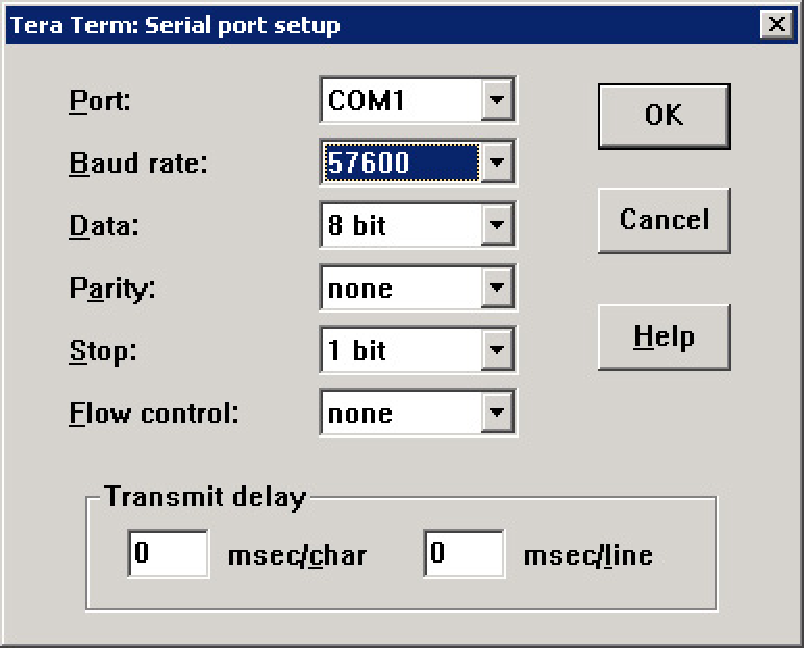
\includegraphics[width=.5\textwidth]{RunScreenshots/EX1p3b.pdf}
	\caption{Step 3 -- Serial Port Settings}
	\label{fig:EX1p3b}
\end{figure}


			
			%Step 4%%%%%%%%%%%%%%%%%%%%%%%%%%%%%%%%%
			\item Tera Term is now ready to receive data.
		\end{enumerate}
		NOTE: (If you are unsure about what rate you choose, this can be found by double-clicking \textbf{RS232} in the \textbf{System Assembly} view. It is the number given for \textbf{UART Lite Baud Rate}). 
	\subsection{Download Peripheral Test to the Board}
		(Assumes that the board has been connected and powered and that the bitstream has been generated successfully)
		
		%Method 1%%%%%%%%%%%%%%%%%%%%%%%%%%%%%%%%%%%%%%%%%%%%%%%%%%%%%%%%%%%
		\subsubsection{Method 1: Directly from XPS}	
			\begin{enumerate}
				%Step 1%%%%%%%%%%%%%%%%%%%%%%%%%%%%%%%%%
				\item Download the bitstream to the board via \textbf{Device Configuration} $\rightarrow$ \textbf{Download Bitstream} or by clicking on the toolbar icon. (NOTE: XPS will recompile/regenerate everything that is not current before downloading the bitstream)
			\end{enumerate}
			
			
\begin{figure}[htbp]
	\centering
		\includegraphics[width=1.00\textwidth]{RunScreenshots/EX2p1p1.pdf}
	\caption{Step 1 -- Download Bitstream}
	\label{fig:EX2p1p1}
\end{figure}

			
		%Method 2%%%%%%%%%%%%%%%%%%%%%%%%%%%%%%%%%%%%%%%%%%%%%%%%%%%%%
		\subsubsection{Method 2: Using iMPACT}
			\begin{enumerate}
				
				%Step 1%%%%%%%%%%%%%%%%%%%%%%%%%%%%%%%%%
				\item Open iMPACT via \textbf{Program Files} $\rightarrow$ \textbf{Xilinx ISE 8.1i} $\rightarrow$ \textbf{Accessories} $\rightarrow$ \textbf{iMPACT}
				
				%Step 2%%%%%%%%%%%%%%%%%%%%%%%%%%%%%%%%%
				\item When the \textbf{iMPACT Project} dialogue box pops up, click \textbf{Cancel} You should see the workspace. 
				
								
\item Right-click on the workspace and choose \textbf{Initialize Chain}. Click \textbf{OK} at the \textbf{Boundary-Scan Chain Contents Summary} window.
				
				%Step 4%%%%%%%%%%%%%%%%%%%%%%%%%%%%%%%%%
				\item You will see the \textbf{Assign New Configuration File} window. Click \textbf{Bypass} for the \textbf{xccace} (first) block.
				
				%Step 5%%%%%%%%%%%%%%%%%%%%%%%%%%%%%%%%%
				\item For the \textbf{xc2vp70} block, browse to the location of your generated bitstream (e.g. ``$\backslash$ProjectFolder$\backslash$implementation$\backslash$download.bit''). Select this file and click \textbf{Open}. Click \textbf{OK} at the \textbf{Add Virtex-II Pro/Virtex-4 Object Files} window to return to the workspace.
				
				%Step 6%%%%%%%%%%%%%%%%%%%%%%%%%%%%%%%%%
				\item Right click on the \textbf{xc2vp70} block, and choose \textbf{Program}. Click \textbf{OK} to download to the board.
			\end{enumerate}
		
		%Method 3%%%%%%%%%%%%%%%%%%%%%%%%%%%%%%%%%%%%%%%%%%%%%%%%%%%%%%%%%%%
		\subsubsection{Method 3: Using ChipScope}
			\begin{enumerate}
				
				%Step 1%%%%%%%%%%%%%%%%%%%%%%%%%%%%%%%%%
				\item Open ChipScope via \textbf{Program Files} $\rightarrow$ \textbf{ChipScope Pro 8.1i} $\rightarrow$ \textbf{ChipScope Pro Analyzer}
				
				%Step 2%%%%%%%%%%%%%%%%%%%%%%%%%%%%%%%%%
				\item Click on the \textbf{Open Cable/Search JTAG Chain} button located in the upperleft corner.
				%Step 3%%%%%%%%%%%%%%%%%%%%%%%%%%%%%%%%%
				\item Click \textbf{OK} at the window that pops up.
				
				%Step 4%%%%%%%%%%%%%%%%%%%%%%%%%%%%%%%%%
				\item Right click on \textbf{xc2vp70} in the box in the upper-lefthand corner. Choose \textbf{Configure}.
				
				%Step 5%%%%%%%%%%%%%%%%%%%%%%%%%%%%%%%%%
				\item Choose \textbf{Select New File} and browse to the location of your generated bitstream (e.g. ``$\backslash$ProjectFolder$\backslash$implementation$\backslash$download.bit'').
				
				%Step 6%%%%%%%%%%%%%%%%%%%%%%%%%%%%%%%%%
				\item Click OK to download to the board.
			\end{enumerate}